\documentclass[11pt]{article}
\usepackage[margin=0.95in]{geometry}
\usepackage{amsmath,amssymb}
\usepackage{tikz}\usepackage{pgfplots}\pgfplotsset{compat=1.18}
\usepackage{xcolor}
\definecolor{ink}{HTML}{1A1B2E}\definecolor{acc}{HTML}{7C3AED}\definecolor{tea}{HTML}{0E9F9A}\definecolor{amb}{HTML}{D97706}\definecolor{ros}{HTML}{E11D48}
\usepackage[colorlinks=true,linkcolor=acc]{hyperref}
\usepackage{titlesec}\titleformat{\section}{\large\bfseries\color{ink}}{\thesection}{.6em}{}
\usepackage{parskip}
\newcommand{\lead}[1]{{\color{acc}\textbf{#1}}}
\usetikzlibrary{arrows.meta,positioning,shapes.geometric}
\begin{document}
\begin{center}{\LARGE\bfseries\color{ink} The Map of the Proof}\\[3pt]{\large\color{acc} What is closed, what is conditional, and exactly where the wall is}\\[2pt]{\small BB(6) research program \quad$\cdot$\quad 2026-09-08}\end{center}
\vspace{4pt}\hrule\vspace{10pt}

\section{The chain, honestly coloured}
\begin{center}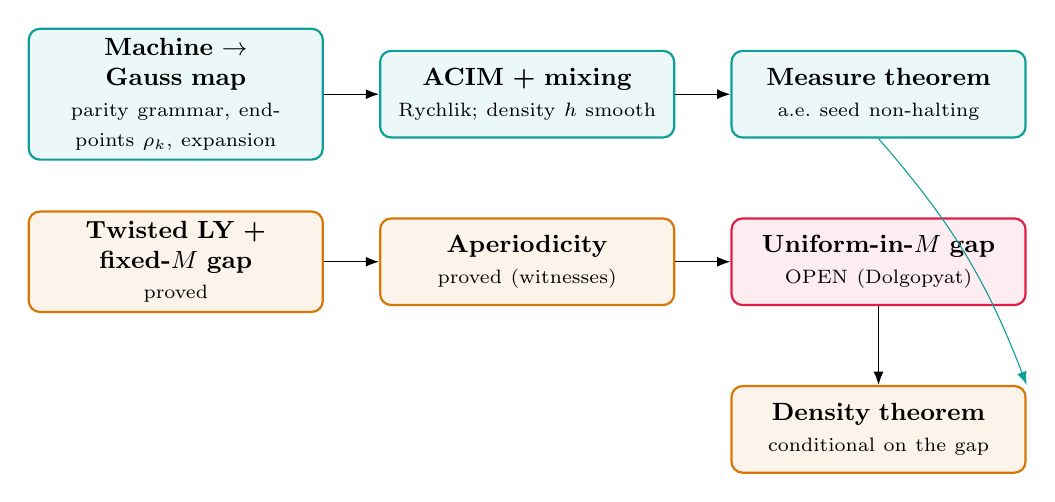
\begin{tikzpicture}[>=Latex,node distance=7mm,every node/.style={font=\small},
box/.style={draw,rounded corners,text width=3.5cm,align=center,minimum height=1.1cm,thick},
ok/.style={box,draw=tea,fill=tea!8},cond/.style={box,draw=amb,fill=amb!8},wall/.style={box,draw=ros,fill=ros!8}]
\node[ok](m){\textbf{Machine $\to$ Gauss map}\\ {\scriptsize parity grammar, endpoints $\rho_k$, expansion}};
\node[ok,right=of m](acim){\textbf{ACIM + mixing}\\ {\scriptsize Rychlik; density $h$ smooth}};
\node[ok,right=of acim](meas){\textbf{Measure theorem}\\ {\scriptsize a.e.\ seed non-halting}};
\node[cond,below=10mm of acim](ap){\textbf{Aperiodicity}\\ {\scriptsize proved (witnesses)}};
\node[cond,left=of ap](ly){\textbf{Twisted LY + fixed-$M$ gap}\\ {\scriptsize proved}};
\node[wall,right=of ap](gap){\textbf{Uniform-in-$M$ gap}\\ {\scriptsize OPEN (Dolgopyat)}};
\node[cond,below=10mm of gap](dens){\textbf{Density theorem}\\ {\scriptsize conditional on the gap}};
\draw[->](m)--(acim);\draw[->](acim)--(meas);
\draw[->](ly)--(ap);\draw[->](ap)--(gap);\draw[->](gap)--(dens);
\draw[->,tea](meas.south) to[bend left=10] (dens.north east);
\end{tikzpicture}\end{center}
\vspace{4pt}
{\small\color{tea}$\blacksquare$ proved \quad}{\small\color{amb}$\blacksquare$ proved, feeds the conditional result \quad}{\small\color{ros}$\blacksquare$ open --- the single wall}

\section{Where every road ends up}
Four independent attacks --- a large sieve, effective equidistribution on a surface, an elementary lattice count, and the transfer operator --- all converge on the \emph{same} spot: controlling the offset when it is small and the scale is large. The sieve is the wrong shape (its moduli $3^{\text{depth}}$ are astronomically large); the surface route fails on non-unimodularity ($\det=\pm3$); the elementary count closes the ``fat'' cylinders but not the thin tail. What is left is one analytic lemma --- a modulus-uniform spectral gap for the twisted operator --- with its hypothesis (aperiodicity) verified, its rate measured favourable, and its two rival routes honestly ruled out.

\section{What this is, and is not}
This is an \lead{almost-all} theorem in the exact sense of Tao's Collatz result: it constrains the generic seed and is silent on any particular one. The certified seed remains Collatz-hard. The measure half is complete; the integer-density half rests on one precisely stated, currently-open estimate. Nothing here is overclaimed --- each downgrade was made the moment scrutiny (including an adversarial review that found a real gap) demanded it.

\vspace{4pt}\hrule\vspace{4pt}\noindent{\small\color{gray} The green path (measure theorem) is unconditional. The amber/red path (integer density) is one Dolgopyat estimate from complete. This is the true state of the program.}
\end{document}